\documentclass[a4paper]{report} % estilo do documento

\usepackage[utf8]{inputenc} %encoding do ficheiro
\usepackage[portuges]{babel} % para língua portuguesa
\usepackage{graphicx}
\usepackage{float}
\usepackage{minted}
\begin{document}

\title{Relatório Trabalho Prático LI1}

\author{Grupo 12\\
\\
José Mendes (A75481) e Ricardo Carvalho (A84261)}
\date{\today}

\maketitle

\tableofcontents

\listoffigures

\listoftables

%% Introdução
\chapter{Introdução}

  \section{Contextualização}
  Este Trabalho foi realizado para a disciplina de LI1 do 1º semestre do ano letivo de 2017/2018.
  Foi pedido aos alunos do curso de Mestrado Integrado em Engenharia Informática que recriassem um jogo originalmente lançado em 1991 pela \textbf{Codemasters}, o  \textbf{Micro Machines.} Este trabalho iria ser feito em duas Fases, e cada Fase teria 3 Tarefas.
  
  \section{Motivação}
   O que nos motivou a fazer este trabalho foi a possibilidade de criarmos um jogo e de também podermos desenvolver a nossa capacidade de programar e de pensar. \par A dificuldade do trabalho acabou por ser mais uma motivação, pois também gostamos de nos desafiar, e acreditamos que essa é a melhor maneira de aprender.
   Acabamos por nos interessar cada vez mais pelo trabalho, visto que ambos gostamos de jogos, de carros e em especial, de programar, e por isso achamos que este foi um trabalho muito importante para o nosso desenvolvimento. 
   
  
  
  
  \section{Objetivos}
Neste trabalho, tínhamos como objetivo recriar o jogo \textbf{Micro Machines} usando Haskell,  de forma a que este pudesse ser jogado contra um \textit{bot}. Ou seja tínhamos não só de fazer um jogo em que pelo menos um utilizador conseguisse jogar, mas também tinha de ser um jogo com um carro que andasse sem indicação de nenhum utilizador ( um \textit{bot}).


  \ldots

%% Análise de Requisitos e Especificação do Problema
\chapter{Análise de Requisitos}
\large Ambas as fases deste trabalho foram divididas em 3 tarefas. Sendo que as primeiras duas tarefas da Fase 1 foram mais para nos ambientarmos a programar visto que não são usadas no decorrer do jogo.\par


\section{Fase 1}
\label{sec:analisefase1}

\large{Esta fase foi dividida em 3 Tarefas, sendo a primeira com o objetivo de criar Mapas, a segunda validar Mapas, e a terceira calcular a trajetória do carro}

\subsection{Tarefa 1}
      Nesta tarefa, foi nos pedido que criasse-mos um programa, capaz de dado um determinado caminho, fosse capaz de criar um Mapa.
      
      
 \begin{minted}{haskell}
constroi :: Caminho -> Mapa
constroi c = Mapa (partida c,Este) t
           where t = 
           preenchertabuleiro (caminhoToPecas 0 (partida c) Este c) 
           (dimensao c) (0,0) c  
\end{minted}

 Tivemos como apoio um Visulaizador de caminhos fornecido pelos professores, e o nosso objetivo era, para qualquer que fosse o caminho dado, conseguir criar um mapa que desse igual ao mapa do visualizador.
 
\subsection{Tarefa 2}
      Nesta tarefa, foi nos pedido para validar um mapa, ou seja, tinhamos de criar um programa que que recebia um mapa, e tinha de determinar se ele era valido ou não.
     
     
     \begin{minted}{haskell} 
      valida :: Mapa -> Bool
valida m = (chegapecapartida list t oi pi) && (tabuleiroSoLava (tabuleiroSemPercurso pos t)) && (rodeadodelava t) && (tabretangulo t) && (orientacaoPecaPartida oi t pi) && (lavaAltura0 (concat t))
         where Mapa (pi,oi) t = m
               list = listaposicoes pi oi t 0 oi pi
               (peca,ori,pos) = separatePecaOrientacaoPosicao (listaposicoes (pi) oi t 0 oi pi)


\end{minted}

    Foi nos também pedido que a nossa função fosse capaz de determinar se o mapa tinha vários caminhos ou apenas um, se o tabuleiro era rodeado por lava ou não e  se as alturas das peças eram compatíveis, e consoante isso, dizer se o mapa era ou não válido.



\subsection{Tarefa 3}
    A Tarefa 3 foi nos pedido algo mais complicado, mas também mais importante, pois era a unica tarefa da 1ª Fase que ia de certeza ser usada na 2ª Fase do trabalho.
    Tinha-mos como objetivo calcular a posição final de um carro, dado a sua posição inicial e a sua Velocidade.
    
  \begin{minted}{haskell} 
      movimenta :: Tabuleiro -> Tempo -> Carro -> Maybe Carro
movimenta m t c = maybecarro
    where Carro posiCar diriCar veliCar = c
          (a,b) = posiCar 
          pospeca = (fromIntegral (floor a), fromIntegral (floor b))
          (posfCar,velfCar) = transitaOuPara (posicaofinal posiCar 
          veliCar pospeca m) posiCar (disttotal veliCar t) veliCar m
          maybecarro = nothingOrJustCar posfCar velfCar diriCar


\end{minted}

     Esta Tarefa deveria devolver um resulado do tipo Maybe Carro , pois o carro teria de ser destruído caso entrasse numa posição lava, e aí o resultado da função seria Nothing.
     Tínhamos também de fazer com que esta nossa Tarefa fosse capaz de calcular a nova direção e velocidade do carro no caso de ele colidir contra alguma parede.
     
     Esta Tarefa foi a nosso ver muito importante pois é a função que no fundo faz com que os nossos carros se possam movimentar.
     
\section{Fase 2}
\label{sec:analisefasee}

\large{Esta fase foi dividida em 3 Tarefas, sendo a primeira (Tarefa 4) com o objetivo desenvolver a Física do jogo e fazer com que o estado dos carros fosse alterado consoante as Ações que estavam  a ser realizadas pelo jogador em questão, na segunda (Tarefa 5) tínhamos de criar a parte visual do jogo , e a terceira (Tarefa 6) tinha o objetivo de criar um \textit{bot} que fosse capaz de se adaptar ás várias circunstancias de uma corrida.}

\subsection{Tarefa 4}

    Nesta tarefa, deveríamos criar uma função que fosse capaz atualizar os vários carros do nosso jogo, mas sem lhes modificar a posição, pois isso já foi algo feito na Tarefa 3 e por isso não deveria ser feito de novo. 
    
      \begin{minted}{haskell} 
    atualiza :: Tempo -- ^ a duração da ação
         -> Jogo  -- ^ o estado do jogo
         -> Int   -- ^ o identificador do jogador
         -> Acao  -- ^ a ação tomada pelo jogador
         -> Jogo  -- ^ o estado atualizado do jogo
atualiza t e j a = Jogo mapa pista carrosAtualiz nitrosAtualiz historicoAtualiz
                 where Jogo mapa pista carros nitros historico = e
                       Propriedades k_atrito k_pneus k_acel k_peso k_nitro k_roda = pista
                       Acao acelera trava esquerda direita nitro = a
                       carrosAtualiz = atualizardirecao e pista k_nitro k_roda t j a nitros carros
                       nitrosAtualiz = acionarNitros j nitros nitro t  
                       historicoAtualiz = atualizaHistorico j e
\end{minted}

   Como esta tarefa apenas recebe uma \textit{Acao}, esta função necessita de ser aplicada varias vezes, de forma a que possa ser aplicada a todos os carros.
   
   As maiores dificuldades causadas por esta tarefa seriam a parte da física que seria necessária para o movimento do carro.

\subsection{Tarefa 5}

 O objetivo desta tarefa é implementar o jogo completo usando a biblioteca Gloss. 
 Esta foi a Tarefa mais livre de todo o jogo. As únicas coisas que deveriam ser obrigatórias eram a parte da corrida, onde deveriam constar pelo menos um carro controlado pelo utilizador e um \textit{bot}.
 Foi nos sugerido pelos docentes da disciplina acrescentar vários extras, entre eles acrescentar menus ao jogo, mais do que um jogador a jogar ao mesmo tempo, e também tentar criar uns gráficos apelativos.
 
 Uma das principais coisas desta tarefa seria de facto a ambientação ao Gloss.

\subsection{Tarefa 6}

Na tarefa 6, tínhamos como objetivo criar um carro que andasse sozinho, seguindo um conjunto de instruções criadas por nós. Este carro deveria ser capaz de se adaptar ás várias circunstancias do jogo.

 \begin{minted}{haskell} 
   bot :: Tempo  -- ^ tempo decorrido desde a última decisão
    -> Jogo   -- ^ estado atual do jogo
    -> Int    -- ^ identificador do jogador dentro do estado
    -> Acao   -- ^ a decisão tomada pelo /bot/
bot tick e j = Acao acel trav esq dir nitro
                   where (dir,esq) = (acaoDirEsq e j)
                         (acel,trav,nitro) = aceleraOuTrava e j tick                      

\end{minted}

Para criar esta tarefa mais interessante e competitiva, foi criado um torneio, para se descobrir qualé, de entre todos os alunos, o \textit{bot} mais rápido a dar uma volta á pista.

%% Descrição da Solução Desenvolvida
\chapter{A Nossa Solução}
\label{sec:solucao}

\section{Fase 1}


\begin{minted}{haskell}

 constroi c == Mapa (partida c,Este) t.

\end{minted}


Tínhamos de criar uma função que a partir de um caminho como argumento devolvesse um mapa.
Para partindo de um caminho construir um mapa resolvemos em primeiro lugar passar o caminho para um conjunto de tuplos composto pela peça e a posição dessa peça correspondentes ao passo efetuado no caminho. Começando-se na posição inicial com uma certa orientação construíamos associávamos a peça de acordo com o passo em questão e com orientação definida de acordo com a orientação da peça anterior. A posição que associávamos à peça era calculada considerando a posição anterior e a orientação a seguir que dependia do tipo de peça anterior e da sua orientação. No final de construir essa lista de posições e peças era preciso preencher o tabuleiro do mapa. Para isso fomos preenchendo linha a linha, posição em posição. Para saber em cada linha se numa determinada posição deveríamos colocar uma peça ou lava verificávamos em cada momento se a posição em que estávamos no tabuleiro estava na lista construida antes com as posições e peças. Se estivesse na lista então colocávamos a peça associada a essa posição, caso contrario colocávamos uma peça do tipo lava. Assim obtivemos o tabuleiro e sabendo a posição e orientação inicial tínhamos então o mapa correspondente ao caminho.    


\section{Fase 2}

    \begin{minted}{haskell}

  valida :: Mapa -> Bool

\end{minted}
    
    Nesta fase era necessário validar um mapa consoante as regras impostas pelos professores, e a função principal apenas recebia como argumento um Mapa. 
    Tivemos de criar um conjunto de Funções cujo resultado seria um booleano, e caso alguma destas funções desse \textit{False}, seria porque houve um dos requisitos para o mapa ser válido que não foi cumprido.
    Dividimos as várias regras de validação em diferentes funções. 
    Criamos uma função que verificava se o mapa é sempre retangular, e para isso tivemos de verificar se o comprimento de cada uma das listas do tabuleiro era ou não igual. Caso isso não acontecesse, o mapa não seria válido. Após isso fizemos também uma função que verificava se um tabuleiro era rodeado por lava, pois essa era outra das regras para um mapa ser válido. Para isso tivemos de verificar se a primeira e ultima linhas e colunas do tabuleiro eram apenas constituídas por peças do tipo Lava.
    Mas não chegava as peças serem do tipo lava, pois tinham de ter altura zero. E por isso decidimos definir uma função que verificasse a altura de todas as peças do tipo Lava, e devolvesse (como nas outras funções) um booleano, consoante o resultado.
    Tínhamos de ver também se um tabuleiro é ou não constituído por apenas um caminho, por isso, após descobrirmos o caminho partindo da peça inicial definida no mapa, retiramos essa caminho e trocamos as suas peças por peças do tipo Lava, e caso ainda houvesse algum tipo Peça que não fosse Lava, é porque existia mais do que um caminho, o mapa não era válido, e por isso a função que tratava desta parte, devolvia um \textit{False}. 
    Depois, tivemos de pensar como resolver o problema da orientação inicial, pois tinha de ser compatível com a peça de partida.  Para isso fizemos uma função que recebia a orientação inicial, o tabuleiro do jogo e a posição inicial, e nesta função tivemos que tratar o caso de todas as curvas e rampas, pois enquanto para uma reta, qualquer direção inicial era válida, para as curvas e para as rampas o mesmo não acontecia, e por isso tivemos de tratar de todos os casos possíveis de serem válidos. Caso aparecesse um caso diferente destes, a função devolvia um \textit{False} e o mapa seria dado como um mapa não válido.
    Nas regras de validação de mapas, foi nos indicado que o percurso deve corresponder a uma só trajetória, tal que começando na peça de partida, com a orientação inicial volta-se a chegar à peça de partida com a orientação inicial, ou seja, tínhamos de verificar que seguindo o percurso correto, não havia hipóteses de acabar num sitio diferente do que começamos, podendo no entanto existir \textit{loops} no mapa.
    Para isso, foi necessário criarmos uma função que a partir da peça e da direção atual, descobrisse a peça seguinte, e isto aplicado de forma recursiva, serviu para verificar se este percurso ia ou não de acabar onde começou.Caso o caminho tivesse diferentes maneiras de ser completado, o mapa ia dar \textit{False} pois iria chumbar na função que testa se todas as peças exceto as do caminho são lava. 
    
   


\section{Fase 3}

 \begin{minted}{haskell}

   movimenta :: Tabuleiro -> Tempo -> Carro -> Maybe Carro

\end{minted}

Nesta fase, os argumentos fornecidos á função principal eram um tabuleiro,  o tempo em que decorria o movimento do carro, e o próprio carro.
Para esta fase apenas tínhamos de calcular a posição final do carro e a sua velocidade ou caso este fosse destruido devolver Nothing. E para saber a posição onde o carro deveria chegar pensamos primeiro em calcular a distancia total que o carro iria andar no espaço de tempo dado caso este fosse sempre em linha reta (a partir do produto do modulo da velocidade com o tempo). Assim caso o carro não fosse destruido teriamos a distancia total que ele iria andar. Sabendo que os pontos criticos de destruição ou colisão ocorriam nos limites das peças então partindo da posição do carro e considerando a velocidade verificavamos se a distancia que ele percorria dessa posição até à posição de limite da peça era menor que a distancia total. Se fosse então paravamos o carro na posição no momento em que a distancia total ficasse zero. Caso fosse maior então faziamos o carro andar até ao limite da peça e verificavamos o que acontecia no limite da peça. Caso fosse destruido então o carro seria imediatamente destruido, se colidisse então era necessário calcular o nosso vetor velocidade de acordo com a a peça em que colidiu. Se ele chegasse a colidir então subtraia-se a distancia percorrida pelo carro à distancia total e voltava-se a verificar se a distancia total era suficiente para chegar ao novo limite da peça. Assim que a distancia total chegasse a zero, caso o carro não tivesse sido destruido, então devolvíamos a velocidade e a posição final resultante do movimento do carro no periodo de tempo.    


\section{Fase 4}

\begin{minted}{haskell}

   atualiza :: Tempo -> Jogo -> Int -> Acao -> Jogo

\end{minted}
Nesta fase criamos um a função que dado um período de tempo, o estado atual do jogo, o identificador de um jogador, e a ação efetuada por esse jogador, atualiza o estado do jogo.
Para atualizar o estado atual do jogo resolvemos atualizar em separado o histórico de posições de cada jogador, a quantidade de nitro disponível para cada jogador e o estado do carro de cada jogador. O mapa do percurso e as suas propriedades não se alteravam pelo que manteve-se os mesmos valores do estado anterior.  Para atualizar o historico de posições do carro dado pelo identificador presente na função principal simplesmente verificarmos se a posição da peça em que o carro que se encontrava estava na no historico de poisições referente a esse mesmo carro. Se já estivesse então mantinha-se inalterada o historico caso contrario acrescentava-se a posição da peça ao inicio da lista do historico. Para atualizar a quantidade de nitro disponivel verificou-se se o jogador, tinha a acção nitro ativada. Se sim então subtraía-se o periodo de tempo entre atualizações ao tempo de nitro disponivel do jogador. Se o tempo entre atualizações fosse maior do que o tempo disponivel então este ultimo valor passava a ser zero. Caso o jogador não tivesse ativado o nitro mantinha-se a quantidade de nitro disponivel como estava no estado anterior. Por fim era preciso atualizar o estado do carro de cada jogador. A posição final do carro não foi alterada devido às condições impostas para entrega do trabalho, mas para ter uma tarefa 4 funcional seria necessário utilizar a fase 3 para obter as posições finais dos carros. A direção do carro do jogador era alterada e para o seu calculo somou-se a direcção atual do carro ao produto do tempo com a constante k_roda. Por fim faltava calcular a nova velocidade final. Para calcular a nova velocidade era necessário somar as forças que estavam ativas no carro. As forças a considerar eram as forças de atrito, de aceleração, da gravidade, da força de pneus e a força do nitro. Todas estas forças foram calculadas a partir da formula dada pelo enunciado referente à fase 2. De notar que todas as forças anteriores eram ativas no carro do jogador exepto a força de nitro, que tanto podia ser ativa nesse mesmo jogador ou então em um adversário. Tendo o vetor velocidade ,do estado anterior do carro, e o vetor soma das forças, somamos esses dois vetores e obtemos a velocidade final do carro. Obtivemos assim o estado final após a atualização.  


\section{Fase 5}
    Esta era a fase mais livre do projeto, pois podíamos escolher o que queríamos incluir no jogo, e tínhamos como objetivo implementar o jogo completo usando a biblioteca Gloss. 
    Começamos por definir como seria o nosso Estado, e decidimos que esta ia conter:
    \begin{enumerate}
   \item Um \textit{Float}, que seria relativo a tempo.
   \begin{itemize}
     \item Este tempo vai ser um constantemente alterado, pela função reageTempo.
   \end{itemize}
   \item Um Int
   \begin{itemize}
     \item Este Int vai servir para o jogo saber se se encontra num menu, ou no jogo em si (parte das corridas).
     \item Este número vai servir também para dar a partida das corridas.
     \item Vai ter de variar dependendo se joga um, ou dois utilizadores.
   \end{itemize}
   \item Duas listas de \textit{Pictures}
   \begin{itemize}
     \item A segunda lista, vai conter todas as pecas do jogo e todos os carros a serem desenhados no ecrã.
     \item a primeira lista vai ser constituída por por pictures da segunda lista, e esta lista vai ser definida pela função mapaparaimagens.
   \end{itemize}
   \item Um tuplo com duas listas de \textit{Pictures} e um \textit{Int}.
   \begin{itemize}
     \item Numa das listas vão se encontrar todas as Pictures relativas aos menus
     \item A outra lista, será apenas constituida por uma \textit{Picture} de cada vez. 
     \item O int vai servir para decidir qual vai ser a picture a ser colocada na lista mais pequena.
   \end{itemize}
   \item Um Jogo
   \begin{itemize}
     \item Este jogo e do tipo data Jogo = Jogo  { mapa:: Mapa, pista:: Propriedades, carros:: [Carro], nitros:: [Tempo], historico :: [[Posicao]]}
   \end{itemize}
   \item Uma lista constituida por 4 elementos do tipo "Acao".
   \begin{itemize}
   \item Cada um destes elementos será relativo a um carro.
   \end{itemize}
   \item Um par de Inteiros.
   \begin{itemize}
   \item Este par vai servir para definir o tamanho da janela e das imagens quando a janela  é aumentada ou diminuída.
   \item Um \textit{Float}.
   \begin{itemize}
   \item Vai servir dar a contagem de inicio da corrida. Começa no zero, e sempre que uma partida é iniciada, começa a aumentar. Chegando a um certo número, os carros são autorizados a partir.
   %%falta um elemneto do estado, mas ainda não esta operacioanal, amanha coloco.
   \end{itemize}
   \end{itemize}
\end{enumerate}
    Aquilo que nós decidimos que o nosso jogo teria de ter era um menu inicial, onde dava para decidir o número de jogadores em jogo. Após este menu achamos que devíamos por uma opção de escolher o mapa do jogo, e para isso fizemos um menu com a base do anterior, mas com a imagem da pista escolhida desenhada no ecrã. Todos os nossos menus recorrem da mesma função, que é uma função que recebe um tuplo (que pertence ao estado) constituído por duas listas de \textit{Pictures} e um número inteiro. Numa destas listas encontram-se todas as pictures relativas a menus, tanto inicias como de escolha de mapas. Na outra das listas vai estar apenas uma imagem, e essa será a imagem a ser desenhada, e quem vai dizer que imagem vai ser desenhada vai ser o número inteiro pertencente ao tuplo dado á função. Este número é apenas alterado na função que reage a eventos.
    Após os menus, tivemos de pensar como passar um tabuleiro para imagens, e para isso criamos uma função recursiva que dado um tabuleiro e dois pares de \textit{Floats} (sendo que o primeiro vai ser relativo a posição de cada uma das pictures, e o segundo vai servir para descobrir a posição da picture seguinte) vai pegar em cada elemento do tabuleiro, e vai lhe associar uma imagem consoante o tipo da peca que é esse elemento. Para esta função é dado também o estado do jogo, de forma a que seja possível ir buscar estas pictures que se encontram no estado.
    Após termos feito a parte dos mapas, começamos por colocar um carro na pista, sendo esse o carro a ser usado pelo utilizador. Começamos por ter o problema de, para o carro andar, termos de estar constantemente a carregar e a soltar as teclas de jogo. Acabámos por resolver esse problema colocando a função que trata do movimento do carro (atualiza da tarefa 4) a ser chamada na função reage tempo, pois essa é uma função que esta constantemente a ser chamada, ao contrario da função reageEvento, que apenas é chamada quando há algum evento novo.
    Após isto, decidimos adicionar o segundo jogador, pois seria igual ao primeiro jogador.
    No entanto, para ser atualizada a função do segundo jogador, juntamente com  a do primeiro, e mais tarde com  a do carro movimentado pela tarefa 6, tivemos de criar uma função que aplicasse não só a atualiza (Tarefa 4), como a movimenta (Tarefa 3). Decidimos aplicar primeiro a atualiza a todos os carros, e so depois a movimenta, poisum carro pode aplicar nitro não apenas a si próprio. Em relação á função movimenta, tivemos de criar uma função decidisse o que fazer com os dados da movimenta, e decidimos que quando essa devolvesse um \textbf{Just}, devolviamos o resultado, mas quando devolvesse um \textbf{Nothing}, usamos o histórico de posições para determinar a peça onde colocar o carro.
    Tivemos também de decidir o que fazer qunado o carro corta caminho ou esta a ir na direção errada, e acabamos por decidir que caso o carro vá na direção oposta ou corte mais do que 3 peças. 
    
    \begin{figure}[H]
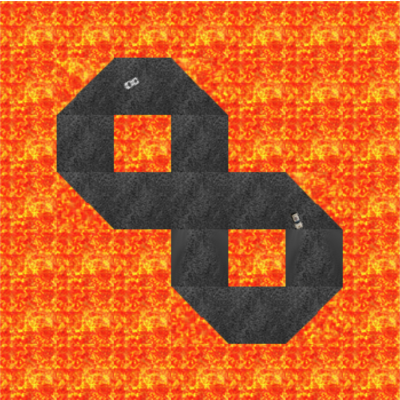
\includegraphics[properties]{imagemT5.png}    
\caption{Imagem da Tarefa 5 }
\end{figure}

    

\section{Fase 6}

\begin{minted}{haskell}

     bot :: Tempo -> Jogo -> Int -> Acao

\end{minted}
    Tinhamos como objetivo definir a função bot, que dada a duração da ação, o estado do jogo e o identificador do jogador, devolve a ação a realizar pelo bot.
	Para descobrir a melhor ação a ser tomada pelo bot resolvemos dividir o problema em dois. Por um lado descobrir a direção que deveria seguir e por outro saber a velocidade ideal em cada momento. Para o problema da direção construimos uma função que iria retornar um tuplo composto pelos booleanos esquerda e direita pertencentes ao data Acao; enquanto para a velocidade a função iria retornar também um tuplo com os booleanos acelerar e travar. Para que o bot soubesse num determinado momento se deveria virar à esquerda ou direita resolvemos primeiro colocar as posições correspondentes ao caminho numa lista, em que as posições se encontravam ordenadas desde a posição inicial até á posição final. Esta ultima função foi aproveitada da tarefa 2. Sabendo construir essa lista fez-se uma função, que dada essa lista e a posição atual do carro, era retornada a próxima posição para onde o carro deveria seguir. Para isso procurou-se a posição da peça em que o carro se encontrava na lista de posições do caminho e retornou-se dessa lista a posição seguinte. No caso de haver entroncamentos teve-se que considerar que na lista iria aparecer duas vezes a mesma posição por isso precisávamos de saber se num certo momento o carro estava a passar pela primeira ou pela segunda vez. Como sabíamos o histórico do carro verificamos se nesse mesmo histórico estava contida a posição a seguir à primeira ocorrência da peça no entroncamento. Deste modo sabíamos que se essa posição seguinte estivesse no histórico então ele já tinha passado uma vez pelo entroncamento e seria a segunda vez que por lá passava. Se não estivesse seria a primeira vez. Assim já se sabia para que peça o carro deveria seguir contudo não tinha nenhuma localização em concreto, não tinha nenhuma posição onde deveria chegar. Para isso definiu-se outra função que dizia a posição a seguir consoante o tipo de peças. Caso fosse do tipo reta ou rampa o carro deveria seguir para a posição referente ao centro da peça. No caso de ser do tipo curva a posição definida seria no "apex" - parte interior da curva, pois teoricamente a melhor linha de corrida é a linha o mais recta possível, e para isso é necessário passar por esse ponto na curva. Tendo assim a posição ideal a seguir, era necessário descobrir se a direção a seguir era de facto a correta. Para isso definimos um ângulo para a linha que continha o posição ideal a seguir e a posição atual do carro (vamos chamar a este ângulo de direção ideal). Sabendo que era dado como argumento na função principal a direção do carro, era possível saber se o angulo da direção atual do carro estava desviado da "direção ideal". Se a direção ideal estivesse num ângulo entre direção atual e  direção atual + 180 então era necessário virar à esquerda. Se fosse num ângulo entre direção atual e direção atual -180 então tinha de virar à direita. Resolvemos comparar com a direção atual e não com a direção da velocidade devido à atualização gradual da velocidade enquanto a direção do carro era atualizada no momento. E assim descobrimos a direção a seguir pelo carro em cada momento.
  Para fazer o carro andar tínhamos de definir se ele devia acelerar, travar ou utilizar nitro. Para saber quais os booleanos a ativar definimos constantes de velocidade do carro para diferentes zonas da pista e para diferentes pisos. Como o gelo tinha uma velocidade de travagem mais baixa os valores de velocidade eram mais baixos enquanto no asfalto e na terra os valores eram mais altos. Estes valores foram obtidos através de experiências. Inicialmente tentou-se construir um modelo que devolvesse valores teóricos de velocidade maximizados mas esta tarefa revelou-se difícil devido à falta de conhecimento na área da matemática que permitisse isso. Os modelos reais da física não puderam se aplicados neste caso, pois o carro não se comportava como um modelo real. As zonas da pista que definimos como importantes foram as retas, as zonas de travagem (quando faltassem x peças para a curva), curvas simples e curvas duplas ou triplas (curvas compostas por duas ou três peças curvas com curvatura sempre para o mesmo lado). Assim quando o carro tivesse mais de x peças retas pela frente ele deveria acelerar. Caso fossem y (em que y>x) peças retas a frente deveria usar nitro. Se tivesse uma curva à frente e a norma da velocidade fosse menor do que a considerada ideal então deveria acelerar. O mesmo acontecia para curvas duplas e triplas sendo a velocidade ideal diferente. Se tivesse um numero pequenos de peças retas à frente então o carro deveria acelerar caso a velocidade fosse inferior a um certo valor. Caso contrario o carro deveria travar. Desta forma nas diferentes zonas da pista o carro conseguia manter as velocidades definidas para esse local. 
    



% Como foi validada a implementação da solução
\chapter{Validação da Solução}

    Para chegarmos ás nossas soluções, fizemos uma variedade de teste em cada uma das funções, desde os testes mais simples aos mais complexos. Nas Tarefas 1,2,3,4,6, fizemos vários testes que tinham como objetivo ter o mesmo resultado que o oracle. 
    Em cada Tarefa fizemos vários testes:
    \begin{itemize}
          \item Testamos Mapas tanto válidos como inválidos na segunda tarefa, e nos inválidos testamos todas as situações possíveis;
    \end{itemize}
 
 \begin{itemize}
    \item Testamos caminhos sem fim, ou com Vários loops na Tarefa 1;
    \end{itemize}
    \begin{itemize}
    \item Criamos o máximo de situações possíveis na Tarefa 3, desde o carro a cair em lava, ao carro a bater contra as paredes inúmeras vezes; 
   \end{itemize}
   \begin{itemize}
    \item Na tarefa 4 testamos com propriedades e com uma combinação diferente de ações de forma a abranger o máximo de situações possíveis;
   \end{itemize}
   \begin{itemize} \item Na sexta Tarefa tentamos experimentar o bot em vários terrenos, e vimos se conseguia fazer várias curvas consecutivas sem bater ou sair da pista. Tentamos também conjugar a utilização de nitro em várias partes do percurso.
   \end{itemize} 
 
    
%Descrever que abordagem tomaram para validar a solução apresentada na Secção \ref{sec:solucao}.

%Em particular pode-se fazer uma descrição dos casos de teste
%realizados para validar o desenvolvimento local.


\chapter{Conclusão}

   A nosso ver, este foi um trabalho muito desafiador e importante para o nosso desenvolvimento e para a nossa compreensão de como funciona o mundo da programação.
   
   Foi claramente um trabalho que desafiou a nossa capacidade de pensar e a nossa criatividade, mas acreditamos que conseguimos corresponder ao desafio lançado.
   Não é fácil desenvolver um jogo em \textit{Haskell}, mas é sem duvida cativante, e por isso ficamos contentes com o resultado final do nosso trabalho, pois pensamos ter conseguido desenvolver um jogo funcional e interessante. 
   
   No fim de tudo ficamos contentes pelo desafio lançado pelos professores, e pela nossa capacidade de resposta perante os problemas encontrados, e esperamos que gostem do nosso trabalho, tanto como nós o gostamos de fazer.
   
   
   

\bibliographystyle{plain}
\bibliography{document}    

\end{document}


